\subsubsubsubsection{Vehicle}
\begin{figure}[h]
\centering
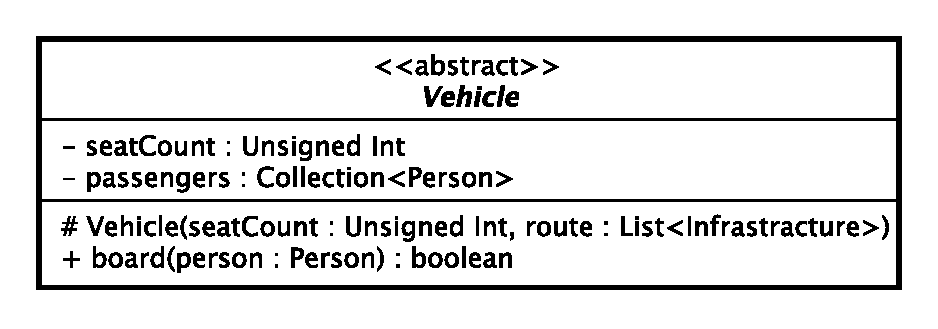
\includegraphics[scale=0.6,keepaspectratio]{images/solution/app/backend/vehicle.eps}
\caption{\pActive::Vehicle}
\label{fig:sd-app-vehicle}
\end{figure}
\FloatBarrier
\begin{itemize}
  \item \textbf{\descr} \\
    It represents an entity that moves through the city carrying one or more
persons.
  \item \textbf{\attrs}
  \begin{itemize}
    \item \texttt{seatCount: Unsigned Int} \\
The number of seats in the vehicle.
    \item \texttt{passengers: Collection<Person>} \\
The collection of passengers carried by the vehicle.
  \end{itemize}
  \item \textbf{\ops}
  \begin{itemize} 
    \item[\#] \texttt{Vehicle(seatCount : Unsigned Int, route : List<Infrastracture>)} \\
Creates a vehicle specifying its number of seats.
    \item[+] \texttt{board(person: Person) : boolean} \\
If the vehicle is not full the person become a passenger and the method 
returns \textit{true}. Otherwise the access to the vehicle is not granted and 
the method returns false.
  \end{itemize}
\end{itemize}
